% ****** Start of file apssamp.tex ******
%
%   This file is part of the APS files in the REVTeX 4.1 distribution.
%   Version 4.1r of REVTeX, August 2010
%
%   Copyright (c) 2009, 2010 The American Physical Society.
%
%   See the REVTeX 4 README file for restrictions and more information.
%
% TeX'ing this file requires that you have AMS-LaTeX 2.0 installed
% as well as the rest of the prerequisites for REVTeX 4.1
%
% See the REVTeX 4 README file
% It also requires running BibTeX. The commands are as follows:
%
%  1)  latex aps25samp.tex
%  2)  bibtex apssamp
%  3)  latex apssamp.tex
%  4)  latex apssamp.tex
%
\documentclass[%
 reprint,
nofootinbib,
%superscriptaddress,
%groupedaddress,
%unsortedaddress,
%runinaddress,
%frontmatterverbose,
%preprint,
%showpacs,preprintnumbers,
%nofootinbib,
%nobibnotes,
%bibnotes,
aps,
%pra,
%prb,
%rmp,
%prstab,
%prstper,
%floatfix,
]{revtex4-1}



\usepackage[utf8]{inputenc}
\usepackage[english]{babel}
\usepackage{dsfont}
\usepackage{amsmath}
\usepackage{ mathrsfs }
\usepackage{amssymb}
\usepackage{graphicx}% Include figure files
\usepackage{dcolumn}% Align table columns on decimal point
\usepackage{bm}% bold math
\usepackage{amsmath}
\usepackage{varioref}
\usepackage{booktabs}
\usepackage[bottom]{footmisc}
\usepackage{minted} % for pseudocode

\usepackage{physics}
\usepackage[ruled,vlined]{algorithm2e}
\usepackage{algpseudocode}
\usepackage{listings}

\usepackage{booktabs}

\usepackage{tikz}
\usepackage{float}
\usepackage{siunitx}



\newcolumntype{C}{>{$}c<{$}}
\AtBeginDocument{
\heavyrulewidth=.08em
\lightrulewidth=.05em
\cmidrulewidth=.03em
\belowrulesep=.65ex
\belowbottomsep=0pt
\aboverulesep=.4ex
\abovetopsep=0pt
\cmidrulesep=\doublerulesep
\cmidrulekern=.5em
\defaultaddspace=.5em
}

\usepackage{ntheorem}
\newtheorem{theorem}{Teorem}
\newtheorem*{theorem-non}{Teorem}
\usepackage{hyperref}% add hypertext capabilities
%\usepackage[mathlines]{lineno}% Enable numbering of text and display math
%\linenumbers\relax % Commence numbering lines

%\usepackage[showframe,%Uncomment any one of the following lines to test
%%scale=0.7, marginratio={1:1, 2:3}, ignoreall,% default settings
%%text={7in,10in},centering,
%%margin=1.5in,
%%total={6.5in,8.75in}, top=1.2in, left=0.9in, includefoot,
%%height=10in,a5paper,hmargin={3cm,0.8in},
%]{geometry}

% \renewcommand{\vec}[1]{\mathbf{#1}} %ny definisjon av \vec så det blir bold face i stedet for vector-pil.

\begin{document}


\title{En videnskablig analyse af den maritime tommelfingerregel for vurderingen af kollisionskurs ved betragtning af baggrundens relative bevægelse til et andet fartøj}
\author{Mikkel Metzsch Jensen}

\affiliation{Department of Physics, University of Oslo\\}
\date{\today}


\begin{abstract}
  In this article we investegate the rule of thumb for recognizing when two boats are on a collision course. The proposed statement to be analyzed, namely \textit{The background method}, can be formulated briefly as: "If the static background seen behind the oncoming boat does not visually move relatively to the boat, then you are on a collision course.". The analysis have shown that this statement is strongly related to the dertermination of the relative bearing. By mathematical derivation we found that if and only if two boats, approaching each other with constant velocity, have constant relative bearing they are on collision couse. Therefore the direct determination of the relative bearing is the most precise way of recognizing a collision course. On the other hand we found that the background method can be used as a means to determine whether the relative bearing is constant in special cases. This were mainly derived by an analytical approach but is also supported by numerical simmulations. In general the background method is found to be valid when used in greater distances to the coast, losely estimated to approximately 833 meters or more. The exact value requires the relative velocity of the observer, the tolerance definition for a humanly recognizable angular velcoty and is dependent on the value of the relative bearning and the angle between the heading and the coast. The nature of this relationship is showcased generally on figure \ref{fig:limit_dimension} and \ref{fig:limit_coastdis}.
\end{abstract}


\maketitle



\section{Introduktion}
Som søfarer findes der en række nødvendige og basale regler, som sikrer god orden og sikkerhed til søs. Heriblandt har vi vigereglerne, som regulerer færdslen på vandet, og forebygger at skibe støder sammen \cite{respektforvand}. Disse regler beskriver som udgangspunkt, hvordan man skal agere, hvis man er på kollisionskurs med andre fartøjer. Det er naturligvis fordelagtigt for søfaren at blive opmærksom på en sådan kollisionfare i så god tid som mulig, så man kan korrigere kurs eller fart. \par
Denne rapport udsprigner af en diskussion med Lars Juel Hansen (sommeren 2020) om en tommelfingerregel for netop vurderingen af kollisionskurs. Denne tommelfingerregel består af en metode, hvorpå iagttageren bruger baggrunden som referanse til at afgøre om man er på kollisionskurs eller ikke. Vi skal fremadrettet kalde den metode for \textit{baggrundsmetoden}, og vi formulerer den som følger.
\begin{quote}
\textbf{Baggrundsmetoden}: Betragt båden som du mistænker en mulig kollision med, og noter et fastliggnede punkt i baggrunden som synes akkurat bag båden. Hvis dette baggrundspunkt i den efterfølgende observationsperiode lader til at flytte sig i forhold til båden, da er du \underline{ikke} på kollisionskurs med båden. Forbliver baggrundspunktet derimod i sigtelinjen bag båden er dette en indikator på at kollisionskursen er reel.
\end{quote}
Ved en undersøgelse af tilgængelige internetkilder findes forskellige gengivelser af denne regel. Ifølge Duelighed.dk \cite{duelighed} kan man ved "betydelige afstande" til kysten bruge observationen om hvordan kollisionsfartøjet trækker "over land" til at vurdere pejlingen til kollisionsfartøjet. Pejlingen er retning fra iagttageren til den genstand, der pejles \cite{ordbog}, og der hævdes i denne sammenhæng:
\begin{quote}
   "[...] fare skal anses for at være til stede, hvis pejlingen af et skib, der nærmer sig, ikke kendeligt forandrer sig." - Duelighed.dk \cite{duelighed}
\end{quote}
Dette kan tolkes således, at hvis den modsejlende trækker mod styrbord i forhold til baggrunden, så vil fartøjet gå styrbord om iagttagerens fartøj. Modsat vil det gå bagbord om iagttagerens fartøj, hvis det trækker til bagbord over land. Hvis ikke fartøjet bevæger sig kendeligt i forhold til baggrunden, vil det indikere at fartøjerne er på kollisionskurs. \par
Dette er i overenstemmelse med baggrundsmetoden, som vi ønsker at undersøge. Dog er det værd at bemærke at metoden fra Duelighed.dk indføres som et middel til at vurdere om der er pejltræk, dvs. om pejlingen til kollisionsfartøjet ændres. \par
I andre kilder (\cite{studienoter}, \cite{retsinformation} \cite{groensund}) er det netop pejlingen, der angives som den direkte indikator på kollisionskurs. Her henvises til en mere direkte fremgangsmåde, for at vurdere om der er pejltræk, ved at anvende et fastliggende punkt på eget fartøj som referanse. Vi vil fremadrettet betegne denne metode som \textit{lokalpunktsmetoden}, og vi formulerer den som følger.
\begin{quote}
\textbf{Lokalpunktsmetoden}: Betragt båden som du mistænker en mulig kollision med, og noter et fastliggnede punkt på eget fartøj (f.eks. et punkt på rælingen), som synes i sigtelinjen til båden. Hvis båden i den efterfølgende observationsperiode lader til at flytte sig i forhold til det lokale punkt, da er der pejltræk, og du er \underline{ikke} på kollisionskurs med båden. Forbliver båden derimod i sigtelinjen for det lokale punkt er dette en indikator på, at der ikke er pejltræk og at kollisionskursen er reel.
\end{quote}
Der fremstår nu to centrale spørgsmål for vurderingen af baggrundsmetodens pålidelighed:
\begin{enumerate}
  \item Hvilken sammenhæng findes der mellem pejltræk til en anden båd og en mulig kollisionskurs.
  \item I hvilken grad kan baggrundsmetoden bruges til at vudere om der er pejltræk.
\end{enumerate}
I denne rapport skal vi fremføre en matematisk analyse af baggrundsmetodens pålidelighed ved at behandle de to overstående spørgsmål. \par
Rapporten bestræber sig på at give en fyldestgørende beskrivelse af det omtalte problem, samtidig som at dette formidles til en målgruppe uden særlig matematisk baggrund. Dette er ikke mulig på alle punkter, da en ordenlig bevisførelse kræver en hvis mængde matematik. Jeg har dog forsøgt at gengive de underliggende resultater og vigtiste pointer undervejs, således at man kan springe beregninger og udledninger over uden at miste kontekst. Dette gælder særlig udledningen i afsnit \ref{sec:pejling_betydning}.


\section{Metode}
\subsection{Definering af problemet}
Vi forestiller os to både til søs, som nærmer sig hinanden. Vi kalder den ene båd for hovedbåden (HB), hvor vi har placeret iagttageren, og den anden båd kalder vi for kollisionsbåden (KB). Vi antager at begge bådene bevæger sig med konstant hastighed, dvs. retlinjet og med konstant fart. Vi beskriver hver båd som et enkelt punkt i et koordinatsystem med akserne $x$ og $y$ som angiver bådens position på vandets overflade set oppefra (se figur \ref{fig:metode_tegning}). Hvis vi kender startpositionen og hastigheden til hver båd, har vi alt den information vi trænger for at beskrive situationen. \par Formelt set kan vi beskrive position $\vec{P} = (x, y)$ som en funktion af tid $t$, når vi kender startposition $\vec{P}_0$ og hastighed $\vec{v}$. For de to både har vi dermed bevægelseslingingen
\begin{align}
  \vec{P}(t) =  \vec{P}_0 + \vec{v}\cdot t
  \label{eq:motion}
\end{align}
Hvis du allerede nu føler en ubehag i kroppen ved synet af ligniner og andre matematiske redskaber, så vil jeg understrege at det holder at tænke på dette som en oversættelse fra ord til tal. Det vigtiste at forstå her, er at vi beskriver bådene som punkter i et koordinatsystem, som bevæger sig i rette linjer med uændret hastighed. \par
Vi definerer en kollision som tilfældet hvor bådene har samme position til samme tidspunkt. I praksis vil man have en kollision allerede hvis bådende passerer tæt forbi hinanden, da bådene naturligvis har en hvis udstrækning i virkeligheden. Dette er dog en uvæsentlig detalje, som ikke bidrager betydnignsfuldt til problemts natur. For at vudere om bådene er på kollisionskurs, er det angiveligt nyttigt at benytte pejlingen. Vi definerer i matematisk forstand pejlingen $\theta_{HB}$ fra HB til KB som vinklen mellem kursen til HB og sigtelinjen fra HB til KB. Dette er illustreret på figur \ref{fig:metode_tegning}.

\begin{figure}[H]
  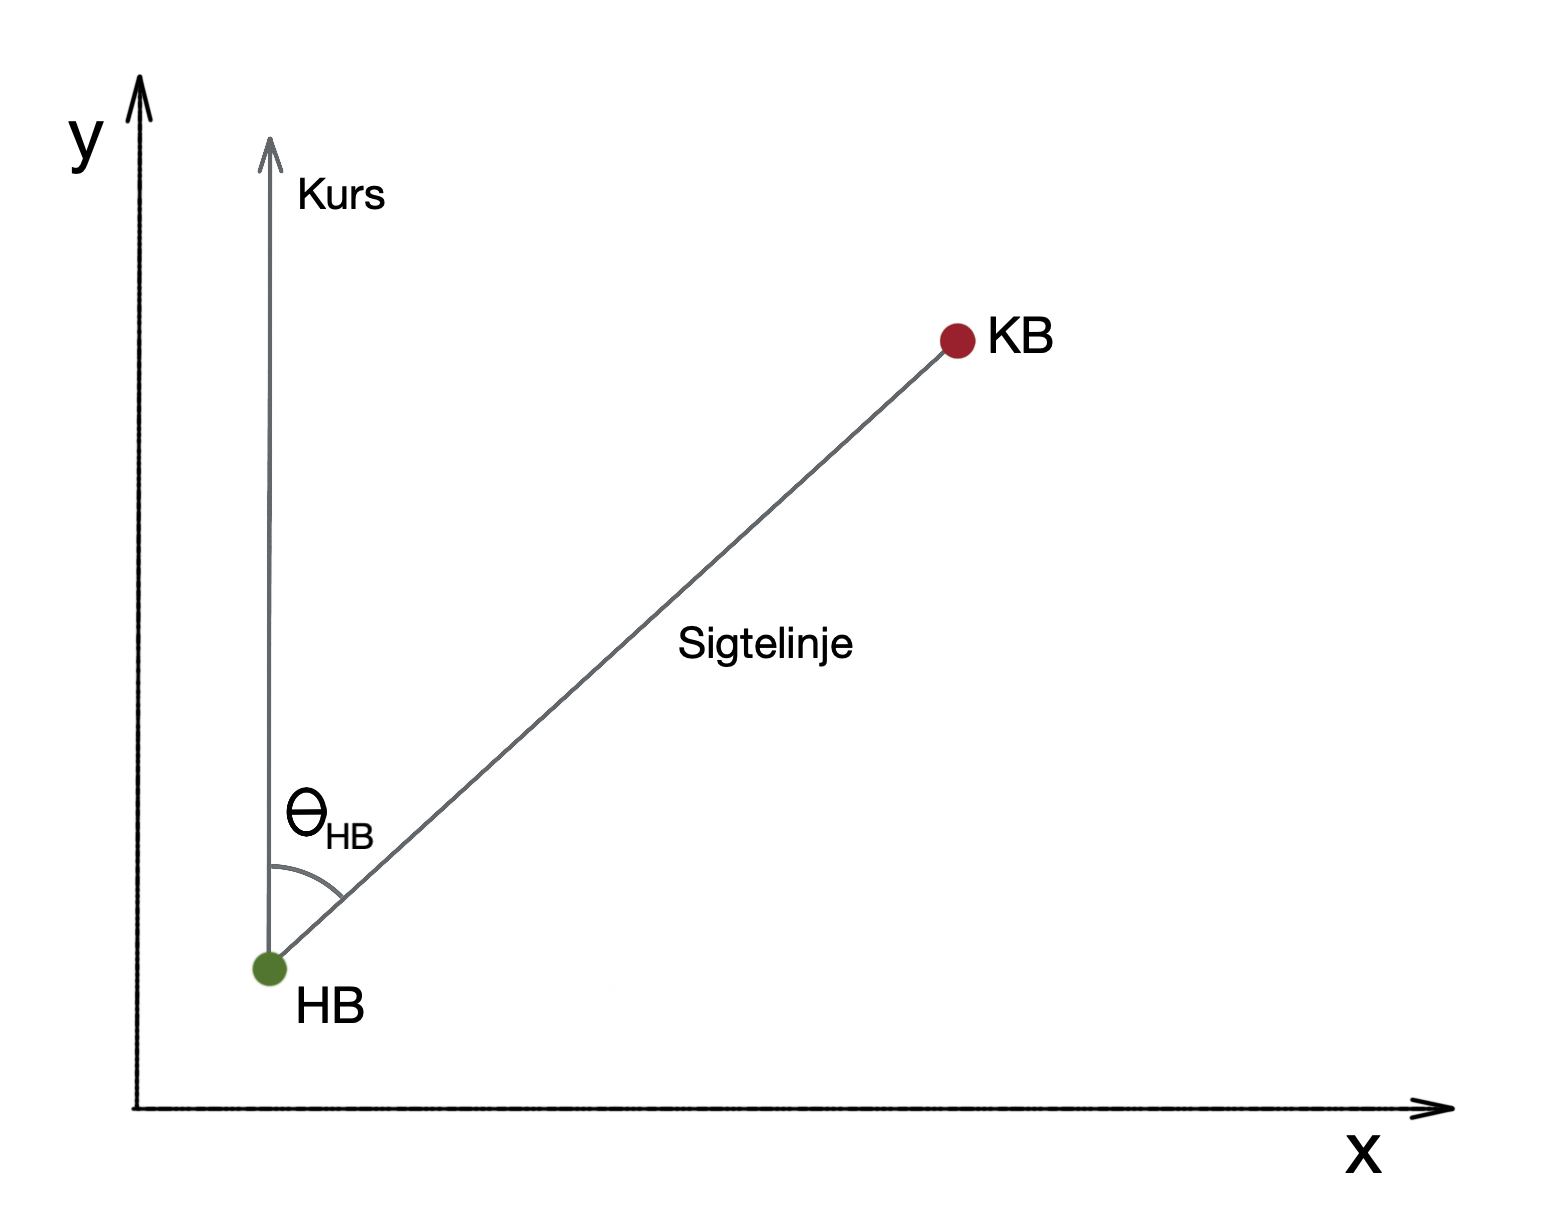
\includegraphics[width=\linewidth]{figures/metode_tegning.png}
  \caption{En illustration af koordinatsystemet som beskriver positionen til de to både på vandoverfladen (set fra oven). Her har vi indtegnet pejlingen $\theta_{HB}$ som defineres som vinklen mellem kursen til HB og sigtelinjen fra HB til KB.}
  \label{fig:metode_tegning}
\end{figure}
Ud fra disse definitioner og indførelselen af et koordinatsystem, er vi klar til at give os i kast med en analyse af situationen under forskellige betingelser.

\subsection{Numeriske simuleringer som støtte til matematiske resultater}\label{sec:numerical_method}
I tillæg til den matematiske analyse, skal vi bruge simple numeriske metoder, måske bedre kendt som simmuleringer, til støtte af vores resultater. \par
For den interesserede kan vi simmulere bådens præcise bevægelse (uden usikkerhed), da alle bevægelserne er lineære. Dette gøres ved at evaluere bevægelsesligning \ref{eq:motion} ved forskellige tidspunkter, analogt til Eulers metode uden acceleration. Vi skriver simmuleringskoden i python som angivet nedenfor. Denne er også tilgængelig på github \cite{github} sammen med diverse scripts for plotting af data.

\begin{minted}[breaklines, breakautoindent = true]{python}
import numpy as np

def simulator(MB_start, OB_start, MB_end, OB_end, T = 10, dt = 0.1):
    K = int(T/dt + 1)         #Steps
    MB_pos = np.zeros((K,2))  #MB = Main Boat
    OB_pos = np.zeros((K,2))  #OB = Other Boat
    t = np.zeros(K)           #Time

    #Initial position
    MB_pos[0] = MB_start
    OB_pos[0] = OB_start

    #Calculate constant velocity
    MB_vel = (MB_end - MB_pos[0])/T
    OB_vel = (OB_end - OB_pos[0])/T

    #Main update loop
    for k in range(K - 1):
        MB_pos[k+1] = MB_pos[k] + MB_vel*dt
        OB_pos[k+1] = OB_pos[k] + OB_vel*dt
        t[k+1] = t[k] + dt
    return MB_pos, OB_pos
\end{minted}


\section{Resultater}
\subsection{Sammenhæng mellem pejltræk og kollisionskurs}
Vi begynder med en intuitiv forklaring på, hvorfor pejltrækket har en helt særlig sammenhæng til kollisionskursen. For at indse denne sammenhæng, skal vi bruge at begge bådende antages at bevæge sig med konstant fart og i en ret linje. Dette har den særlige egenskab, at en iagttager på HB også vil se at KB bevæger sig med konstant fart og i en ret linje relativt til iagtagerens perspektiv. Når vi skifter perspektiv, siger vi i fysikkens verden, at vi skifter koordinatsystem eller mere formelt intertialsystem. Mens koordinaterne $(x, y)$ angiver positionen på vandet ud fra et fikseret referansepunkt, så kan vi skifte til koordinatsystemet med koordinaterne $(x',y')$ som angiver position relativt til HB. I dette koordinatsystem vil HB altid være placeret i origo, med koordinat $(0,0)$, og de andre både beskrives ved positionen relativt til HB. Det betyder at hvis HB bevæger sig fremad i $(x,y)$-systemet så vil stillestående punkter fra dette system bevæge sig bagud i $(x',y')$-systemet. På figur \ref{fig:reference_frame_explainer} ses hvordan koordinaterne til en række bådruter ændres ved overgangen fra det "normale" $(x,y)$-system til $(x',y')$-systemet. Brug gerne et øjeblik på at studerer overgangen vist på figur \ref{fig:reference_frame_explainer}, da det er konceptuelt vigtig for den følgende forklaring.

\begin{figure}[H]
  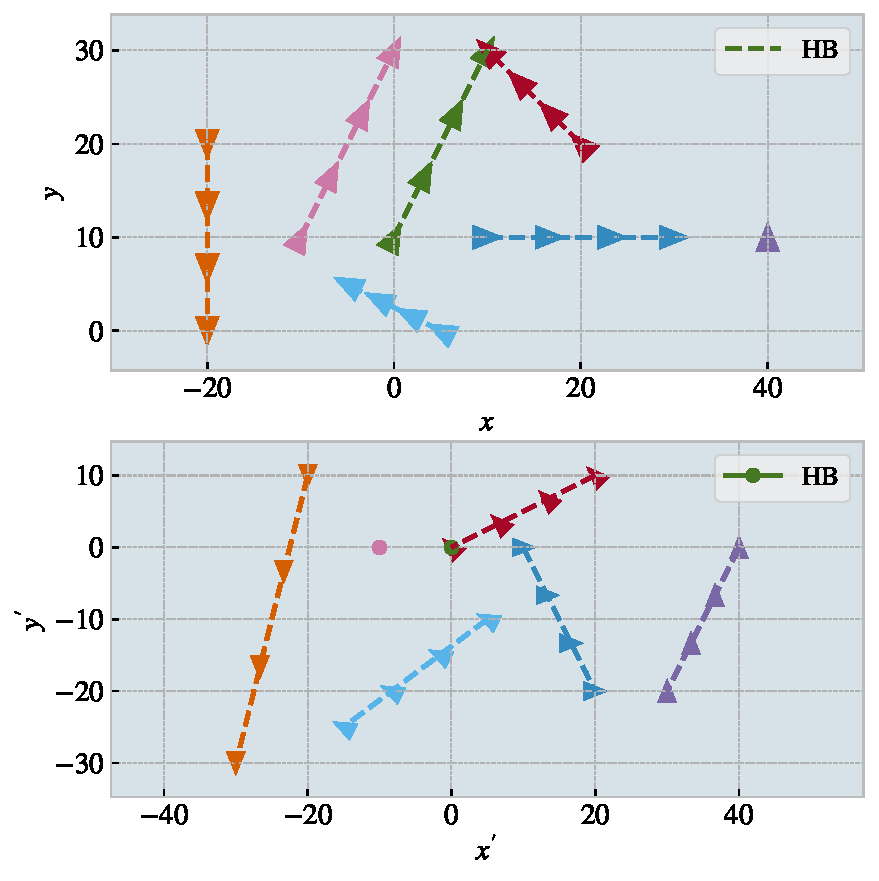
\includegraphics[width=\linewidth]{figures/reference_frame_explainer.pdf}
  \caption{En illustration af ændringen fra koordinatsystemet $(x,y)$ til HB's intertialsystem med koordinaterne  $(x',y')$ for en række bådruter. Pilens retning angiver bådens kurs og vi ser i $(x',y')$-system at bådene ikke følger pilens retning, og dermed ser ud til at sejle sidelæns eller baglæns. Dette skyldes naturligvis netop at HB selv flytter sig. Bemærk for eksempel at den lille båd som egentlig står stille i $(x,y)$ nu bevæger sig i  $(x',y')$. Tilsvarende står den lyserøde båd i ro i $(x',y')$ fordi den bevæger sig parallelt (og med samme fart) som HB. }
  \label{fig:reference_frame_explainer}
\end{figure}

Som det fremgår af figur \ref{fig:reference_frame_explainer}, vil enhver bevægelse være retlinjet i $(x',y')$-systemet, dersom bevægelserne er retlinjet i det orginale $(x,y)$-systemet. Dermed ved vi, at hvis KB kolliderer med HB, så kan vi tegne dette som en ret linje med endepunkt i origo $(0,0)$ i $(x',y')$-systemet. Dette er netop tilfældet for den røde båd på figur \ref{fig:reference_frame_explainer}. Faktisk kan vi med dette udgangspunkt definere kollisionskursen ved at KB rammer origo i $(x',y')$-systemet. Dette medfører i tilfældet med kollisionskurs, at en iagttager på HB nødvendigvis vil se at KB bevæger sig direkte mod iagtageren. Dette er den eneste mulige rette linje hvorpå bådene kan kollidere uden at medparterne ændrer retning eller fart undervejs. På figur \ref{fig:reference_frame_explainer2} ser vi hvordan forskellige kollisionsruter alle rammer origo i $(x',y')$-systemet.

\begin{figure}[H]
  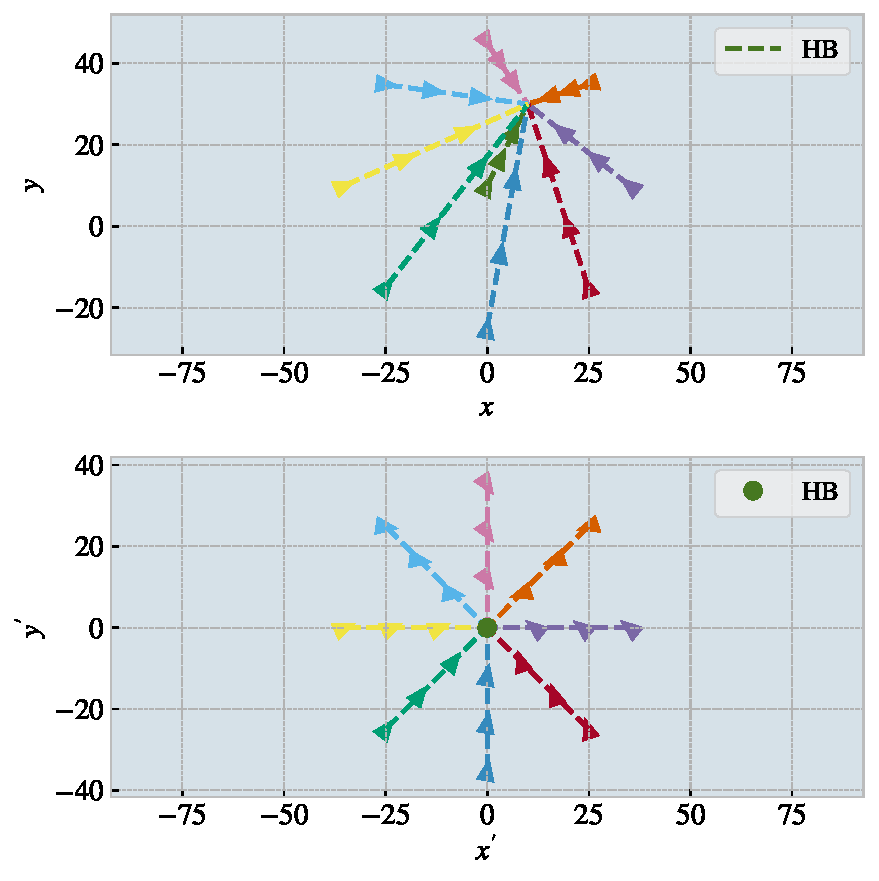
\includegraphics[width=\linewidth]{figures/reference_frame_explainer2.pdf}
  \caption{Forskellige kollisionsruter i både $(x,y)$- og $(x',y')$-systemet. Uanset hvilken retning kollisionsbåden kommer fra i $(x,y)$-systemet, vil det medføre at båden rammer origo i $(x',y')$-systemet.}
  \label{fig:reference_frame_explainer2}
\end{figure}

Som iagtager på HB, vil man altså i alle disse tilfælde med kollision, se at pejlingen til bådene er uændret indtil kollisionen. Derfor vil en iagtager ikke opleve pejltræk for kollisionsbåden. De eneste andre situationer hvor pejlingen er konstant er når bådene begge ligger stille, sejler parallelt eller sejler væk fra hinanden på en bestemt måde. For disse tre tilfælde nærmer bådene sig dog ikke i afstand, og det er dermed enkelt at afgøre, at der ikke er kollisionsfare i disse tilfælde. Altså når vi frem til delkonklusionen:

\begin{quote}
Hvis bådene nærmer sig hinanden, og der ikke er noget pejltræk, da er bådende på kollisionskurs.
\end{quote}

I det følgende afsnit skal vi give en matematisk udledning for overstående konklusion. Med matematisk støtte kan vi formulere den lidt mere formelt, som det ses i det vi kalder teorem \ref{Teo:pejling}. Hvis du ikke er til matematik, så kan du trygt springe næste afsnit over, da det ikke bidrager mere til problemet, men blot bekræfter det vi allerede har argumenteret for i det overstående. Hvis du ikke køber argumenterne over, så er næste afsnit essentielt.


\subsection{Sammenhæng mellem pejltræk og kollisionskurs (matematisk udledning)}\label{sec:pejling_betydning}
Med grundlag i argumenterne fra forrige afsnit, skal vi nu give en mere grundig udledning, for at en uændret pejling, til en båd som nærmer sig, er ensbetydene med kollision. Da vi har antaget at bådene bevæger sig med konstant hastighed, kan vi bruge en lineær transformation til HB's intertialsystem $(x',y')$. Positionen $\vec{P}'_{KB}$ til KB i det nye intertialsystem kan skrives:
\begin{align*}
  \vec{P'}_{KB}(t) &= \vec{P}_{KB}(t) - \vec{P}_{HB}(t) \\
  &= \vec{P}_{0,KB} + \vec{v}_{KB}t - \vec{P}_{0,HB} - \vec{v}_{HB}t \\
  &= (\vec{P}_{0,KB} - \vec{P}_{0,HB}) + (\vec{v}_{KB} - \vec{v}_{HB})t \\
  &= \vec{P'}_{0,KB} + \vec{v'}_{KB}t
\end{align*}
Vi ser som forventet at $\vec{P}'_{KB}$ også beskriver en retlinjet bevægelse. I tilfældet hvor bådene er på kollisionskurs ved vi at $\vec{P}'_{KB}(t_k) = \vec{0}$ ved kollisionstidspunktet $t_{k}$. Dette medfører sammenhængen:
\begin{align}
  \vec{P'}_{0,KB} &= - \vec{v'}_{KB}t_k \nonumber \\
  \begin{pmatrix} x'_{0,KB} \\ y'_{0,KB} \end{pmatrix}\frac{1}{t_k} &=   -\begin{pmatrix} v'_{x,KB} \\ v'_{y,KB} \end{pmatrix}
  \label{eq:P=v}
\end{align}
% \begin{align}
%   \vec{P'}_{0,KB} &= - \vec{v'}_{KB}t_k \nonumber \\
%   (x'_{0,KB}, y'_{0,KB})\frac{1}{t_k} &= -(v'_{x,KB}, v'_{y,KB})
%   \label{eq:P=v}
% \end{align}
Vi kan da finde pejlingen $\theta_{HB}$ ved at omskrive $\vec{P}'_{KB}$ til polære koordinater. Her er vi bare interesseret i vinkelkoordinat $\phi_{KB}$ der bestemmes som
\begin{align*}
  \phi_{KB}(t) &= \arctan{\left( \frac{y'(t)}{x'(t)}\right)} \\
  &= \arctan{\left( \frac{y'_{0,KB} + v'_{y,KB}t}{x'_{0,KB} + v'_{x,KB}t}\right)}
\end{align*}
Vi bruger da sammenghængen fra ligning \ref{eq:P=v} og finder
\begin{align*}
  \phi_{KB}(t) &= \arctan{\left( \frac{y'_{0,KB} - y'_{0,KB}\frac{t}{t_k}}{x'_{0,KB} - x'_{0,KB}\frac{t}{t_k}}\right)} \\
  &= \arctan{\left(\frac{y'_{0,KB}}{x'_{0,KB}} \frac{1 - \frac{t}{t_k}}{1 - \frac{t}{t_k}}\right)} \\
  &= \arctan{\left(\frac{y'_{0,KB}}{x'_{0,KB}}\right)} = \text{konst.} \\
\end{align*}
Fra dette ser vi at vinkelkoordinat $\phi_{KB}$ er konstant (uavhængig af tid), hvilket medfører at pejlingen også er konstant:
\begin{align*}
  \theta_{HB} &= \frac{\pi}{2} - \phi_{KB} = \text{konst.}
\end{align*}
Fra dette ræsonoment, har vi altså vist at pejlingen vil være konstant, i tilfældet hvor bådene er på kollisionkurs. Hvis bådene følger kollisionskursen men i modsat retning (bevæger sig væk fra hianden), kan vi indføre betingelsen $\vec{P}'_{KB}(t_i) = \vec{0}$ for et tidspunkt $t_i < 0$. Derved kan vi opstille en ligning tilsvarende \ref{eq:P=v} og derved finde at pejlingen også vil være konstant i dette tilfælde. Hvis ikke bådene er på kollisionskurs er ligning \ref{eq:P=v} ikke længere gyldig og $P'_{KB}$ kan tage hvilken som helst retlinjet bane uden om $\vec{P}'_{KB} = \vec{0}$. Det betyder at $\phi_{KB}$ og dermed også pejlingen $\theta_{KB}$ vil ændre sig som funktion af tid. Dette fører i sidste ende til slutningen:
\begin{theorem}
  Hvis og bare hvis to både med konstant hastighed, som nærmer sig i afstand, har konstant pejling til hinanden er disse på kollisionskurs.
  \label{Teo:pejling}
\end{theorem}


\subsection{Falsifisering af baggrundsmetoden}
Vi har nu fastslået, at pejltrækket kan bruges som en direkte indikator på om bådene er på kollisionskurs eller ikke. Vi kan derfor allerede nu bekræfte at lokalpunktsmetoden vil være en pålidelig metode for påvisning af kollisionskursen. Spørgsmålet som genstår nu, er hvorvidt baggrundsmetoden er en god metode til at vurdere pejltrækket. Vi skal altså undersøge, om der er sammenfald mellem pejltræk og baggrundens bevægelse relativt til sigtelinjen gennem KB. \par
I tilfældet med kollisionskurs ved vi fra teorem \ref{Teo:pejling} at sigtelinjen fra HB gennem KB vil have en konstant vinkel. I det enkle tilfælde hvor kystlinjen er relinjet og parallel med kursen til HB vil sigtelinjens skæring med kystlinjen forflytte sig med samme hastighed som HB. Dette resultat bekræftes og illustreres godt ved simuleringen vist på figur \ref{fig:eks1}.
\begin{figure}[H]
 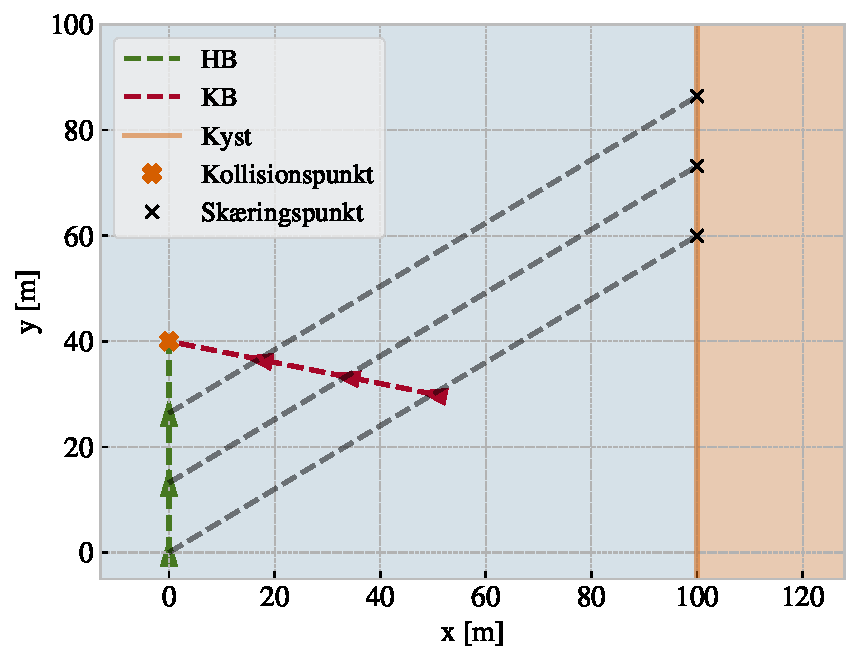
\includegraphics[width=\linewidth]{figures/eksempel1.pdf}
 \caption{En simulering af bådene HB og KB på kollisionskurs, med kollisionspunkt 100 meter fra kysten. Her plottes fire positioner for bådene (inklusiv kollisionspunktet) jævnt fordelt i tid. Fra de grå stiblede linjer ser vi hvordan sigtelinjen fra HB gennem KB skærer med kystlinjen ved de forskellige tidspunkter. Dette skæringspunkt forflytter sig som forventet i henhold til HB's bevægelse.}
 \label{fig:eks1}
\end{figure}
I situationen på figur \ref{fig:eks1}, bevæger HB sig 40 meter frem i løbet af simmuleringen, hvilket medfører at sigtelinjen fra HB til KB forskydes tilsvarende 40 meter op langs kysten (i positiv y-retning). Det betyder at en iagtager på HB i samme tidsrum vil se at et referansepunkt på kysten bevæger sig 40 meter i modsat retning. HB befinder sig her kun 100 meter væk fra kysten, og derfor vil en relativ forflyting af referansepunktet på 40 meter højst sandsynlig være kendelig. I denne situation, er baggrundsmetoden derfor vildledene, og en iagtager på HB vil fejlagtigt tro at situationen er ufarlig. Vi har altså med dette ene eksempel modbevist at baggrundsmetoden ikke virker i alle tilfælde. Vi kalder formelt set dette for en falsifering af teorien. I appendix \ref{sec:appendix} ses flere simmulerigner for en række situaitoner med og uden kollision. Her ser vi både eksempler hvor baggrundspunktet forflytter sig relativt ved kollision, og eksempler hvor baggrundspunktet ser ud til at være stillestående (i en kort periode) uden kollision. \par
Spørgsmålet er om der findes nogle kriterier, for hvilke baggrundsmetoden alligevel kan bruges som en pålidlig indikator på kollisionskursen.



\subsection{Grænsebetingelser for brug af baggrundsmetoden}
Vi begynder med undersøgelsen af hvordan afstanden til baggrunden (kysten) spiller en rolle for baggrundsmetodens pålidlighed. Hvis vi modifiserer det omtalte eksempel (på figur \ref{fig:eks1}), således at kollisionspunktet flyttes en kilometer væk fra kysten, da vil baggrundens forflytning på kun 40 meter højst sandsynlig ikke klassifiseres som en kendelig forflytning. I et sådan tilfælde vil baggrunden altså synes at være stillestående, og dermed vil baggrundsmetoden være en udmærket indikator for kollisionskursen. Vi skal i det følgende kvantifisere dette og estimere en mulig grænse for hvornår baggrundsmetoden kan bruges forsvarligt. \par
Fra HB's perspektiv vil baggrundspunktet (BP) som nævnt bevæge sig med en fart tilsvarende HB's egen fart men modsat vej. Vi husker på at et stillestående punkt i $(x,y)$-systemet bevæger sig modsat af HB når vi beskriver det i $(x',y')$-systemet. Matematisk set kan vi skrive dette som
\begin{align*}
  \vec{v'}_{BP} = - \vec{v}_{HB}
\end{align*}
Det betyder, at en iagtager på HB, som betragter baggrundspunkt BP vil se at pejlingen til BP ændres med en vinkelhastighed som vi kalder $\omega_O$. Vinkelhastigheden beskriver hvor hurtigt en vinkel ændres, og dermed hvor meget pejltræk vi har over tid. Matematisk beregenr vi vinkelhastigheden som
\begin{align*}
 \omega_O = -\frac{v_{HB}\sin{(\theta_{HB})}}{d}
\end{align*}
hvor $v_{HB} = |\vec{v}_{HB}|$ er HB bådens fart langs kursen, $\theta_{HB}$ er pejlingen til KB (og dermed BP), og $d$ er afstanden til kysten/BP via sigtelinjen. Se figur \ref{fig:grænsebetingelser_illustration} for illustration af situationen. Bemærk at vi i praksis skal antage at baggrundspunktet ligger akkurat på kystlinjen, og ikke længere inde på landområdet.

\begin{figure}[H]
  \includegraphics[width=\linewidth]{figures/grænsebetingelser_illustration.png}
  \caption{Illustration af situationen, hvor vi noterer et baggrundspunkt (BP) i sigtelinjen til KB. Her baggrundspunket ikke placeret præcis på kystlinjen, selvom vi fremadrettet skal bruge denne antagelse, og derfor vil snakke om afstanden til baggrundspunktet og kysten ved baggrundspunktet som en og samme ting.}
  \label{fig:grænsebetingelser_illustration}
\end{figure}

Vi definerer minimumsgrænsen for en kendelig forflytning ved vinkelhastigheden $\omega_k$. Vi kender ikke værdien af denne, men den skal beskrive den mindste bevægelse som vi er i stand til at opfange. I praksis må vi da også tage hensyn til, at det er mere udfordrende at opfange små bevægelser i urolige omgivelser til søs, og at metodens grænse ikke bør baseres på urimelige fintfølende observationer. Med kendskab til denne grænseværdi $\omega_k$, vil kriteriet for en kendelig bevægelse være givet ved uligheden:
\begin{align}
 |\omega_O| &< \omega_k \nonumber \\
 \frac{v_{HB}|\sin{(\theta_{HB})}|}{d} &< \omega_k \nonumber \\
 \frac{v_{HB}|\sin{(\theta_{HB})}|}{\omega_k} &< d
 \label{eq:limit}
\end{align}
Vi kan da bruge denne sammenhæng til at finde den minimale afstand $d$ for brug af baggrundsmetoden som funktion af $\theta_{HB}$. Dette resultat er vist på figur \ref{fig:limit_dimensionless}.
 \begin{figure}[H]
   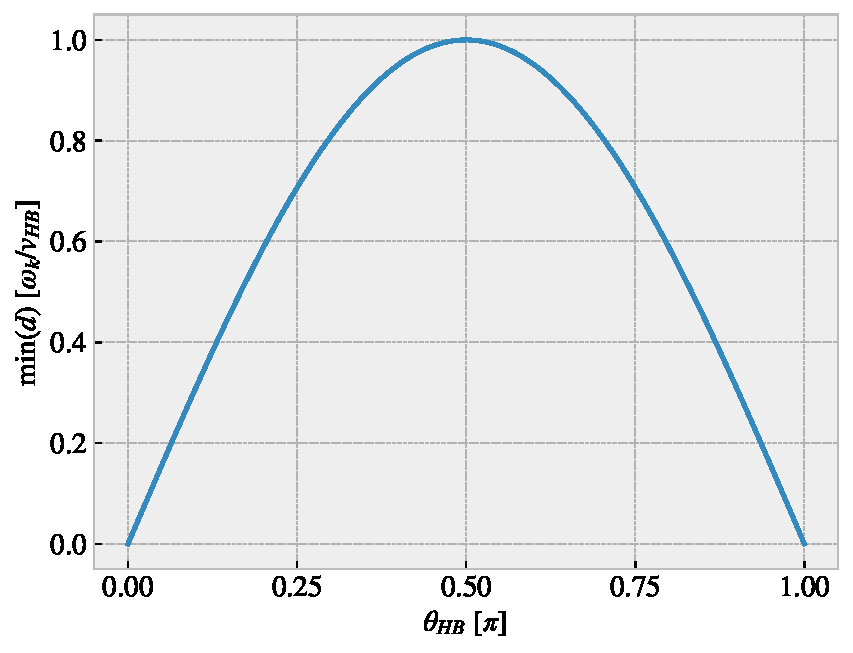
\includegraphics[width=\linewidth]{figures/limit_dimensionless.pdf}
   \caption{Den minimale afstand $\min{(d)}$ som funktion af pejlingen $\theta_{HB}$ som mulliggør brug af baggrundsmetoden. $d$ beskriver afstanden til kysten via sigtelinjen. Resultatet er angivet med dimensionløse enheder med skaleringsfaktorene $\omega_k$ som er den minimale vinkelhastighed for en kendelig forflytning og $v_{HB}$ som er farten til HB. For at baggrundsmetoden skal være anvendelig, må vi kræve at $d$ ligger over kurven for $\min{(d)}$.}
   \label{fig:limit_dimensionless}
 \end{figure}
Resultatet på figur \ref{fig:limit_dimensionless} er i matematisk forstand et fint generelt resultat, da det giver den nødvendige information og baggrundsmetodens gyldighed ved forskellige pejlingsvinkler, hastigheder til HB og ikke mindst forskellige kriterier for hvad en kendelig forflytning er. Dog er den svær at tolke direkte, da tallene på y-aksen ikke giver nogen intuitiv mening. Som fysiker ville vi nok have stoppet her, men vi skal i det følgende prøve at tolke på det generelle resultat ved at lave en række antagelser på de ukendte værdier i problemet. Dog er det værd at bemærke at kurvens top på $\theta_{HB} = 0.50 \ \pi$ fortæller os at baggrundsmetoden vil kræve den største afstand til kysten når pejlingen til KB er på $90^{\circ}$, altså vinkelret på kursen til HB. Desto nærmere vinkelen kommer at være parallel med kysten desto mindre bliver den nødvendige kystafstand for brug af metoden. Dette skal vi se nærmere på i det følgende.

\subsection{Tolkning af det generelle resultat for grænsebetingelser}
For at klargøre betydningen af det generelle fra figur \ref{fig:limit_dimensionless}, har vi brug for at sætte tal på hvad en kendelig forflytning er. Indtilvidere har vi defineret dette med kritiske vinkelhastighed $\omega_k$, og vi skal nu bruge en række kvalificerede gæt for at estimere værdien af denne. Bemærk at følgende resultater derfor bygger på en del usikkerheder.

\subsubsection{Estimering af kritiske vinkelhastighed}
Vi forestiller os, at vi ved observation af KB vil benytte et centralt punkt på båden som referanse mod baggrunden. En mulig defintion på en kendelig forflytning kan derfor være at baggrundspunktet har flyttet sig ud til eller forbi kanten af båden i løbet af en observationsperiode. Observationsperioden kan vi sætte til 10 sekunder, svarende til den nedre grænse af tidsintervallet 10-20 sekunder som nævnes i \cite{duelighed}. Vi siger da at forflytningen er kendelig hvis baggrundspunktet har flyttet sig en relativ afstand større eller lig halvdelen af bådens tværlængde (set fra iagttagerens perspektiv) i løbet af de 10 sekunder. For sejlbåde i den lidt større klasse kan vi bruge en gennemsnitlig bredde på 5 m og længde på 15 m, hvilket giver 10 m som middelestimat (tilsvarer at vi gjennemsnitlig ser båden fra en 45 graders sigtelinje). Til sidst må vi også bestemme den afstand der er mellem bådene når kollisionsrisikoen vurderes. Hertil bruger vi 200 meter som en minimumsværdi. Ud fra disse antagelser finder vi at den kritiske vinkelhastighed for en kendelig forflyting kan defines som:
\begin{align}
  \omega_k = \frac{\arctan{(\frac{1}{2}\frac{10 \text{m}}{200 \text{m}})}}{10 \text{s}} = 0.0025 \ \text{s}^{-1} \approx  0.14^{\circ}\ \text{s}^{-1}
  \label{eq:omega_k}
\end{align}
Dette estimat giver os en ide om størrelsen på den kritiske vinkel, og vi skal tage udgangspunkt i denne værdi for de videre beregninger. Bemærk at vi har valgt de overstående værdier på en sådan måde at de effektivt set giver et maksimums estimat for $\omega_k$ og dermed et minimumsatimat for den gyldige afstand $d$. Altså har vi valgt tallene sådan at vi giver baggrundsmetoden de bedst mulige vilkår for vores videre analyse. \par
% Som det fremgår af det overstående, har vi altså virkelig gang i gætteværktøjet nu, men disse antagelser gøres udelukkende for estimere menneskets evne til at kende en forflytning i praksis. Hvis denne værdi kunne hentes fra faktiske studier vil det være at foretrække. I tillæg har
%
Vi kan nu bruge at en typisk bådhastighed er 4 knob, hvilket tilsvarer omtrent 2 m/s. Med disse værdier kan vi skalere resultatet fra figur \ref{fig:limit_dimensionless}, sådan at vi får det nye resultat på figur \ref{fig:limit_dimension} med mere meningsfyldte enheder.
\begin{figure}[H]
  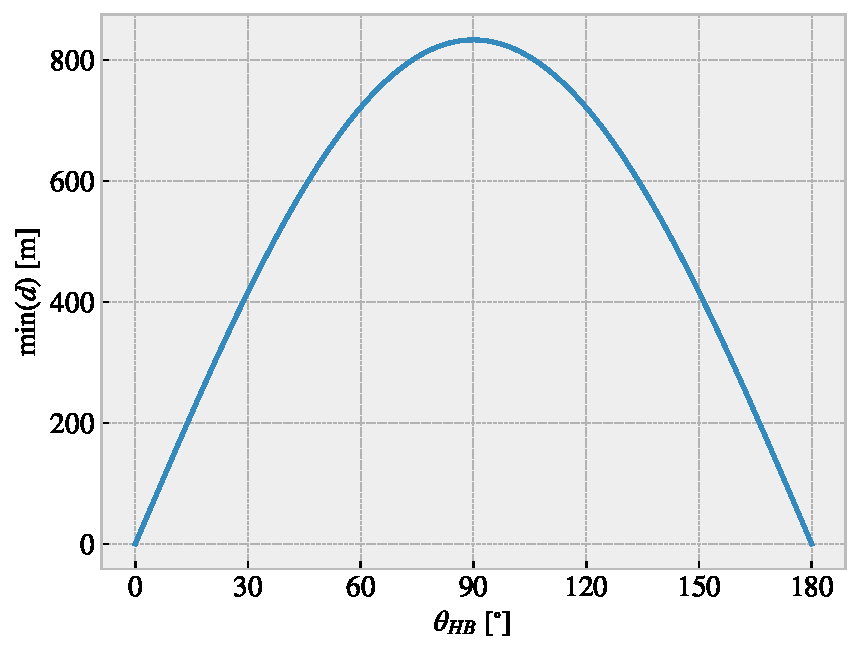
\includegraphics[width=\linewidth]{figures/limit_dimension.pdf}
  \caption{Den minimale afstand $\min{(d)}$ som funktion af pejlingen $\theta_{HB}$, som mulliggør brug af baggrundsmetoden. $d$ beskriver afstanden til kysten via sigtelinjen i meter. Enhederne er fastlagt ud fra figur \ref{fig:limit_dimension} med brug af estimaterne $\omega_k = 0.14^{\circ}\ \text{s}^{-1}$ og $v_{HB} = 2 \ \text{m/s}$.}
  \label{fig:limit_dimension}
\end{figure}
På figur \ref{fig:limit_dimension} kan vi nu aflæse afstanden $d$, som vi husker er afstanden langs sigtelinjen til BP, som funktion af pejlingsvinklen. For eksempel vil det kræve at afstanden til BP er større eller lig $d\approx 830$ m ved en pejlingsvinkel på $90 ^{\circ}.$, og dermed at man i et sådan tilfælde må befinde sig omtrent $830$ m eller længere væk fra kysten for at baggrundsmetoden er gyldig. Har vi i stedet en pejlingsvinkel på $30 ^{\circ}.$ skal vi have at $d$ er større eller lig  $d\approx 420$ m. Siden vi i sidste tilfælde har en pejlingsvinkel forskellig fra $90 ^{\circ}.$ betyder det at vi kan befinde os endnu tætere på kysten end bare 420 m. Det er altså derfor ikke helt intuitivt at aflæse det gyldige område i form af en direkte afstand til kysten/baggrunden. Vi kan derfor omregne resultatet den korteste afstand til kysten. \par
I en situation hvor den retlinjede kyst har en vinkel $\beta$ i forhold til HB's kurs kan vi omregne afstanden $d$ langs sigtelinjen til den korteste afstand $s_{\text{kyst}}$ mellem HB og kysten (linjen vinkelretpå kysten). Omregning gøres som
\begin{align}
  s_{\text{kyst}} = d\cdot \sin{(\theta_{HB} + \beta)}
  \label{eq:s_kyst}
\end{align}
Ved at anvende denne omregning får vi resultatet vist på figur \ref{fig:limit_coastdis}.
\begin{figure}[H]
  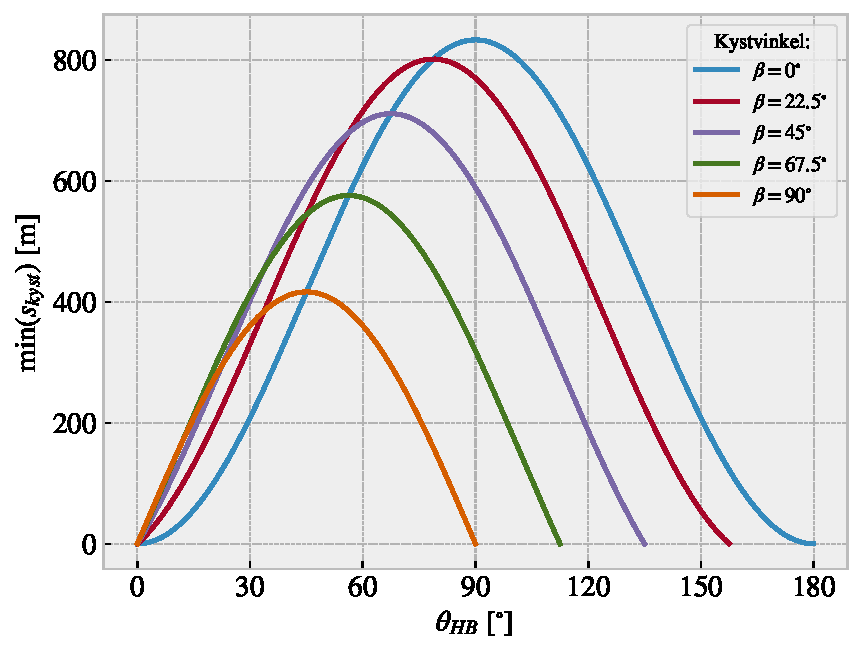
\includegraphics[width=\linewidth]{figures/limit_coastdis.pdf}
  \caption{Den minimale afstand til kysten $\min{(s_{\text{kyst}})}$ som funktion af pejlingen $\theta_{HB}$, som mulliggør brug af baggrundsmetoden. $s_{\text{kyst}}$ (se ligning \ref{eq:s_kyst}) er den korteste afstand for HB til kysten, når kysten har en vinkel $\beta$ i forhold til HB's kurs.}
  \label{fig:limit_coastdis}
\end{figure}
Resultatet på figur \ref{fig:limit_coastdis} giver os nu mulighed for at aflæse den minimume afstand til kysten som kræves i en givet situation baseret på pejlingsivnkel $\theta_{HB}$ og kystvinkel $\beta$. \par
I praksis er det dog lettere omstændigt at tage hensyn til kystvinklen og vi kan derfor eliminere kystvinkelsafhængighet ved at vælge den kystvinkel som giver den største afstand $s$. Vi kan tænke på dette som en sammensmeltning af alle graferne for de forskellige valg af $beta$, hvor vi da har taget den største værdi herfra (dette illustereres på figur \ref{fig:limit_coastdis_betamax}). Vi husker på at
\begin{align*}
  s_{kyst} = d\cdot \sin{(\theta_{HB} + \beta)} \propto \sin{(\theta_{HB} + \beta)}
\end{align*}
og derved ser vi at vi opnår maksimalværdi ved at vælge $\beta = \frac{\pi}{2} - \theta_{HB}$. Da finder vi at den maksimale værdi som funktion af $\theta_{HB}$ forenkles til
\begin{align}
  \max{[s_{kyst}]}(\theta_{HB}) = d
  \label{eq:max_s_kyst}
\end{align}
Det viser sig at denne forenkling akkurat tilsvarer samme graf som vi fik på figur \ref{fig:limit_dimension}. På figur \ref{fig:limit_coastdis_betamax} ses hvordan valg af $\beta = \frac{\pi}{2} - \theta_{HB}$ netop indeholder kurverne for alle andre valg af $\beta$.
\begin{figure}[H]
  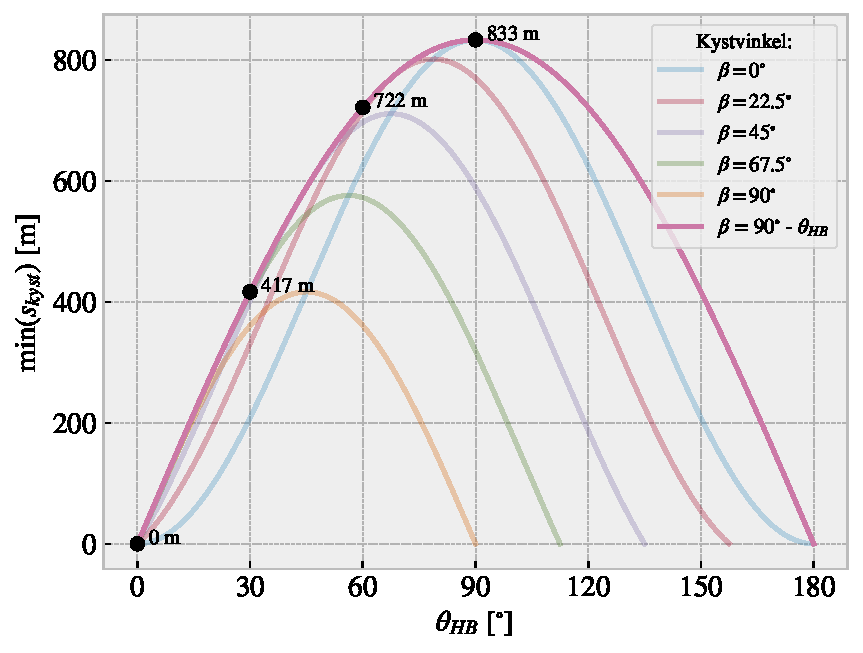
\includegraphics[width=\linewidth]{figures/limit_coastdis_betamax.pdf}
  \caption{Den minimumme afstand $\min{(s_{kyst})}$ som funktion af pejlingen $\theta_{HB}$ som muliggør brug af baggrundsmetoden (se figur \ref{fig:limit_coastdis}). Den lyserøde kurve for $\beta = 90^{\circ} - \theta_{HB}$, tilsvarerer det valg af $\beta$ for hvert punkt som giver den største værdi. Dermed har vi et maksimumsestimat på $\min{(s_{kyst})}$ som kan aflæses uavhængig af kystvinkel $\beta$ }
  \label{fig:limit_coastdis_betamax}
\end{figure}

\subsection{Numeriske simuleringer}
Ved brug af koden vist i afsnit \ref{sec:numerical_method} har vi simmuleret forskellige situationer for at understøtte de matematiske resultater. I appendix \ref{sec:appendix} findes en række resultater fra forskellige situationer med og uden kolliosionskurs. I tillæg findes en række animationer på github'en \cite{github}, som giver et mere intuitiv indblik i bevægelserne, og hvordan pejling og baggrundspunkt forflyttes. Vi ser generelt at simmuleringerne er i overenstemmelse med de matematiske resultater.


\section{Diskussion}
Ud fra den matematiske slutning om pejlingen i teorem \ref{Teo:pejling}, er det klart at pejlingen kan bruges som en direkte indikator på kollisionskurs. Hvis KB nærmer sig og pejlingen ikke ændres er dette ensbetydene med at bådene vil kollidere, givet at kurs og retning fastholdes. Altså vil lokalpunktsmetoden være troværdig i alle situationer og derfor også være den bedst egnede metode. \par
Som antydet på Duelighed.dk \cite{duelighed}, fandt vi også at baggrundsmetoden kan bruges som en indikator på om der er pejltræk eller ikke givet visse betingelser. I tilfælde med konstant pejling, vil baggrunden flytte sig tilsvarende HB's relative bevægelse til baggrunden. Siden denne relative bevægelse bliver mindre og mindre tydelig desto længere væk fra den observerede baggrund man befinder sig, kan baggrundsmetoden effektivt anvendes ved større afstande til kysten. Dette er i overenstemmelse med påstanden fra Duelighed.dk \cite{duelighed}. Med kendskab til den minimale vinkelhastighed $\omega_k$ for en kendelig forflytning, samt HB's hastighed, kan man kortlægge det gyldige område for baggrundsmetoden via det generelle resultat fra figur \ref{fig:limit_dimensionless}. Med kvalificerede gæt estimerede vi $\omega_k = 0.14^{\circ}\ \text{s}^{-1}$, og ved antagelsen om HB's fart på $v_{HB} = 2$ m/s, kom vi frem til det mest alsidige specifikke resultat på figur \ref{fig:limit_coastdis}. Her ser man hvordan den gyldige afstand til kysten (baggrunden) afhænger af pejlingsvinkel $\theta_{HB}$ og kystvinkel $\beta$. Dog er det endelige maksimumsresultat på figur \ref{fig:limit_coastdis_betamax}, med alle kystvinkler taget i betragtning, mere anvendelig for sejlere i praksis. Ved aflæsning af denne figur finder vi blandt andet punkterne vist i tabel \ref{tab:valid_area}.
\begin{table}[H]
 \begin{center}
 \caption{Aflæsning af punkter på figur \ref{fig:limit_coastdis}.}
 \begin{tabular}{|c|c|} \hline
 $\theta_{HB}$ [$^{\circ}$] & $s_{kyst}$ [m]  \\ \hline
 0 & 0 \\ \hline
 30 & 417 \\ \hline
 60 & 722  \\ \hline
 90 & 833 \\ \hline
 \end{tabular}
 \end{center}
 \label{tab:valid_area}
\end{table}
Aflæsningen af denne tabel giver et hurtigt overblik af det gyldige område for baggrundsmetoden. Her ser vi at baggrundsmetoden kan bruges tættere på kysten når KB pejles med spids vinkel, mens en pejling på 90 $^{\circ}$ vil være det mest kyst-afstanskrævende sted at anvende metoden. \par
Som en sidste note nævner vi muligheden for at baggrundsmetoden kan anvendes hos en erfaren søfarer. Hvis søfaren har erfaring med hvordan bagrundens relative forflytning opleves ved forskellige pejlingsvinkler og bådhastigheder, kan søfaren vurdere om baggrunden bag en modsejlende båd ændres mere eller mindre end dette. Altså er det muligt, at søfaren selv kan korrigere for den forflytning som skyldes søfarens egen bevægelse i forhold til baggrunden. Dog kræver det et godt kendskab til forskellige kollisionssituationer, og det er diskutabelt om metoden stadig kan siges at være i brug i dette tilfælde. Uanset vil lokalpunktsmetoden være et mere oplagt valg, dersom man er i tvivl om en eventuel kollisionskurs.
\linebreak


\newpage

\section{Konklusion}
Fra den matematiske udledning kan vi konkludere at pejlingen kan bruges som en direkte indikator på kollisionskurs. Når to både nærmer sig hinanden, med konstant hastighed, vil pejlingen mellem skibende være konstant hvis disse er på kollisionskurs. Dette medfører at lokalpunktsmetoden (se indledning) vil være en god metode i alle tilfælde. \par
Vi fandt dog, at baggrundsmetoden kan bruges som en indirekte metode til at bestemme om bådene er på kollisionskurs, hvis iagttageren befinder sig tilstrækkelig langt væk fra baggrunden. Når bådene er på kollisionskurs, hvilket medfører konstant pejling, vil baggrunden bag kollisionsbåden forflytte sig med samme hastighed som iagttagerens relative hastighed til baggrunden. Ved længere afstande til kysten er denne forflytning ikke kendelig, og derved vil baggrunden opleves at være i ro. Resultatet fra figur \ref{fig:limit_dimensionless} giver den mest generelle angivelse af det gyldige område for brug af baggrundsmetoden. Ikke desto mindre fandt vi ved brug af en række estimater for kendelig forflytning og bådhastighed, at afstanden til kysten som kræves for at anvende baggrundsmetoden kan estimeres med sammenhængen vist på figur \ref{fig:limit_coastdis_betamax}. Den største afstand som kræves er her approksimeret til 833 m ved en pejling på 90 $^{\circ}$, mens det ved en pejlingen på 30 eller 150 $^{\circ}$ er 417 m. Det er dog vigtigt at understrege at disse estimater som formidler det generelle resultat fra figur \ref{fig:limit_dimensionless} er baseret på usikre antagelser. Dette bør derfor kun tolkes som et estimat på størrelsesordnen for denne grænse.





\begin{thebibliography}{9}
  \bibitem{github} Metzsch-Jensen M. (2020), \textit{Boat myth} (GitHub repository), tilgængelig ved: \url{https://github.com/mikkelme/boat_myth}

  \bibitem{respektforvand} Respekt for vand: \textit{Vigeregler}, tilgængelig ved: \url{https://soesport.dk/sejlskolen/vigeregler} (sidst læst: 16/01/2021)

  \bibitem{duelighed} Duelighed.dk: \textit{Skipper-kursus} (slide 03-02), tilgængelig ved: \url{http://www.duelighed.dk/tutorial_soevejsregler/03_02.htm} (sidst læst: 05/01/2021)

  \bibitem{ordbog} Hjemmeværnet: \textit{Maritime udtryk}, tilgængelig ved: \url{https://www.hjv.dk/oe/HVF122/Sider/Maritime-udtryk.aspx} (sidst læst: 05/01/2021)

  \bibitem{studienoter} Søren Toftegaard O. (2013), \textit{LystSejlads}, s. 19 (afsnit 1.4) , tilgængelig ved: \url{http://studienoter.dk/Sejlads/Noter/LystSejlads.pdf} (sidst læst: 05/01/2021)

  \pagebreak
  \bibitem{retsinformation} retsinformation.dk: \textit{Bekendtgørelse om søvejsregler} 20/11/2009. Regel 7: fare for sammenstød (d) (20/11/2009), tilgængelig ved: \url{https://www.retsinformation.dk/eli/lta/2009/1083} (sidst læst: 05/01/2021)

  \bibitem{groensund} Albrechten S. (2007). \textit{Sejlads for Begyndere} \url{http://www.groensund.dk/upl/website/sejlads/SejladsforBegyndere2.pdf}


\end{thebibliography}

\clearpage
\onecolumngrid
\section{Appendix}\label{sec:appendix}

\subsection{Simmuleringer med kollision}

\begin{figure}[H]
  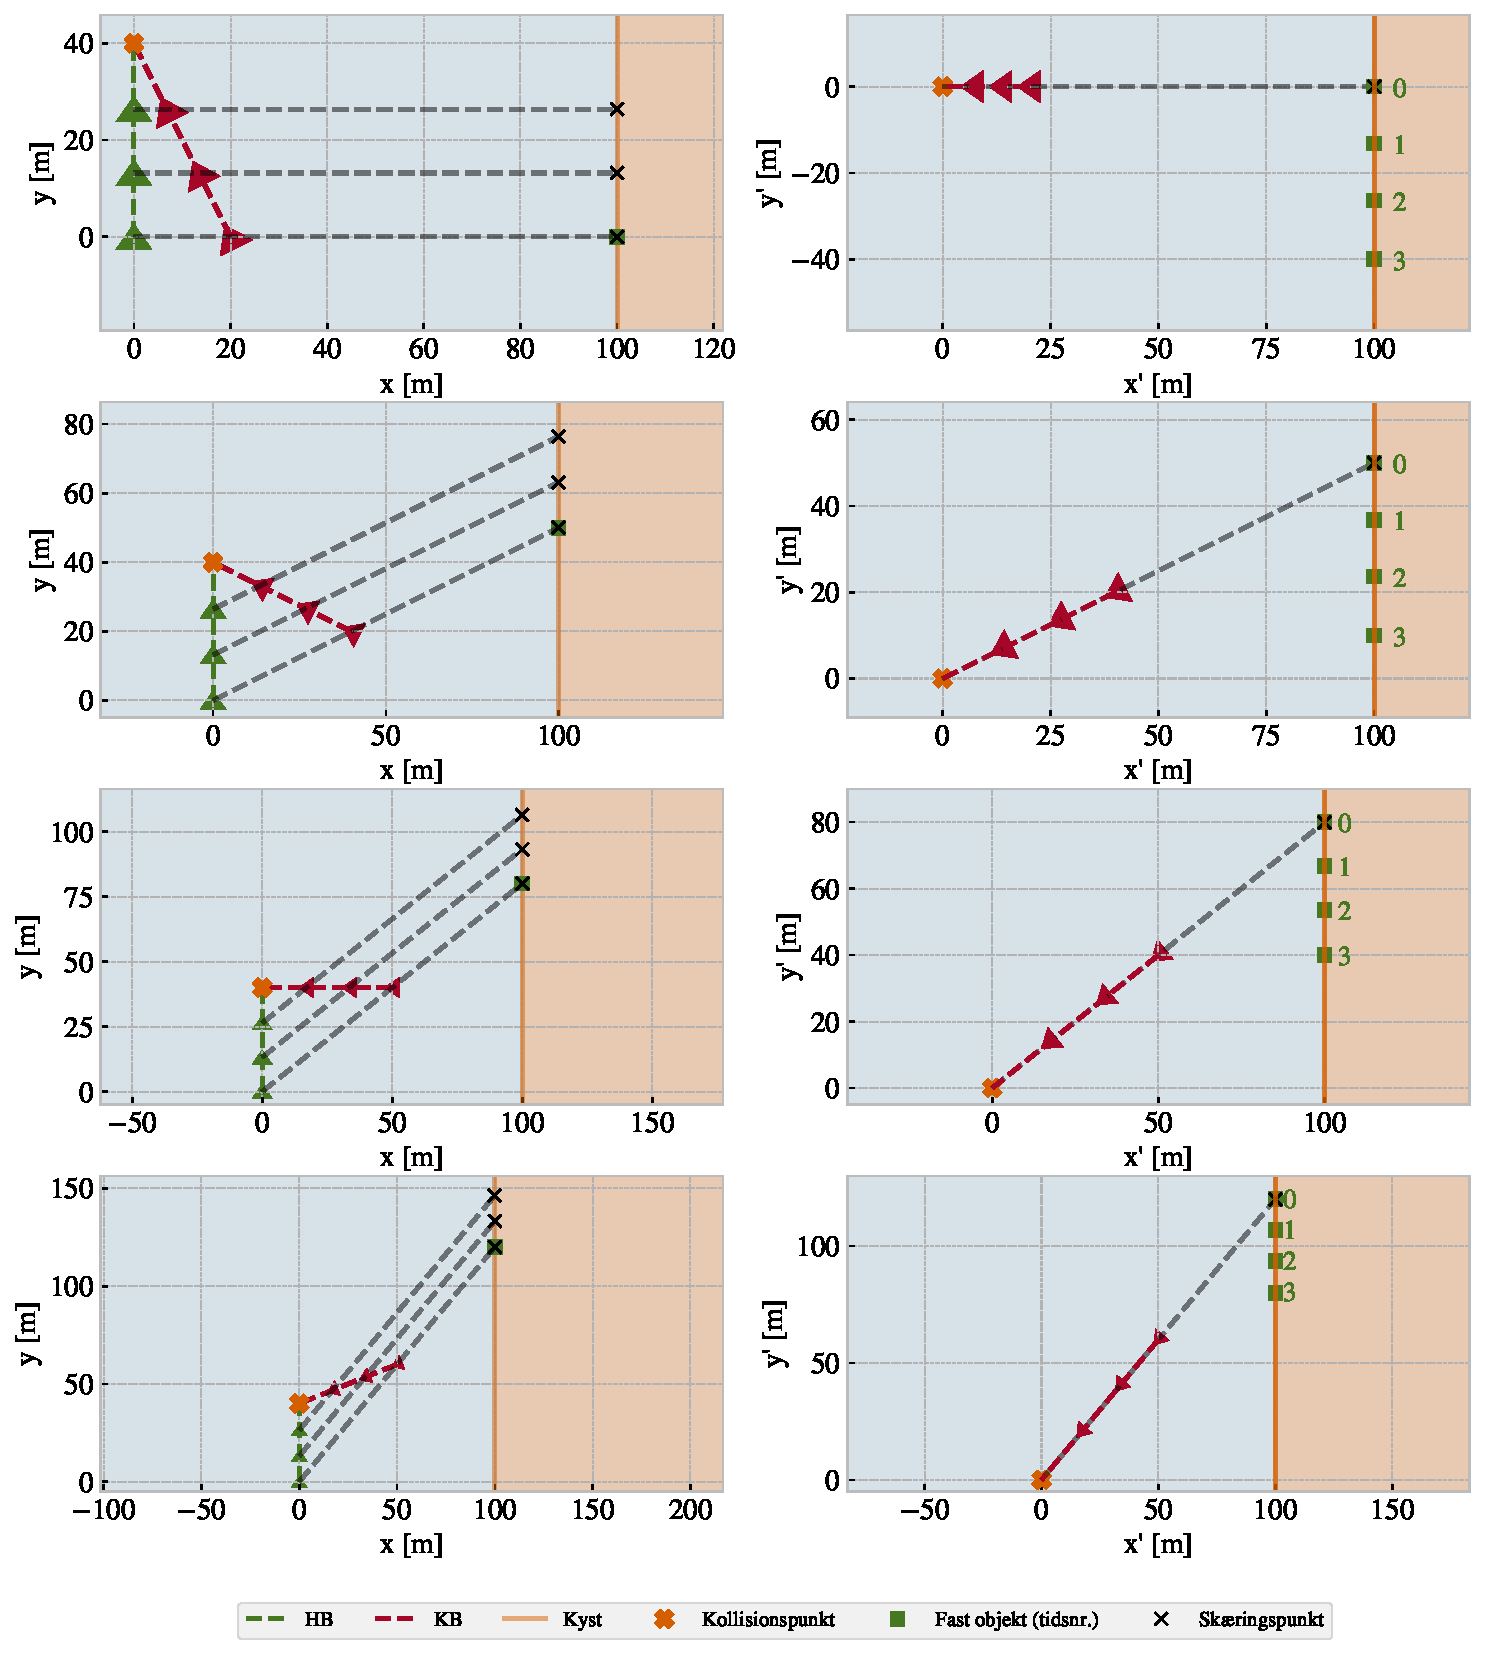
\includegraphics[width=\linewidth]{figures/subplot_C1.pdf}
  \caption[A table inside a caption]{
\begin{tabular}{|c|c|c|c|c|}
\hline
Figurrække & $HB_{start}$  & $KB_{start}$ & $HB_{slut}$ & $KB_{slut}$\\ \hline
1  & (0,0) & (20,0) & (0, 40) & (0, 40) \\ \hline
2  & (0,0) & (40,30) & (0, 40) & (0, 40) \\ \hline
3  & (0,0) & (50,40) & (0, 40) & (0, 40) \\ \hline
4  & (0,0) & (50,60) & (0, 40) & (0, 40) \\ \hline
\end{tabular}}
  \label{fig:subplot_C1}
\end{figure}

\begin{figure}[H]
  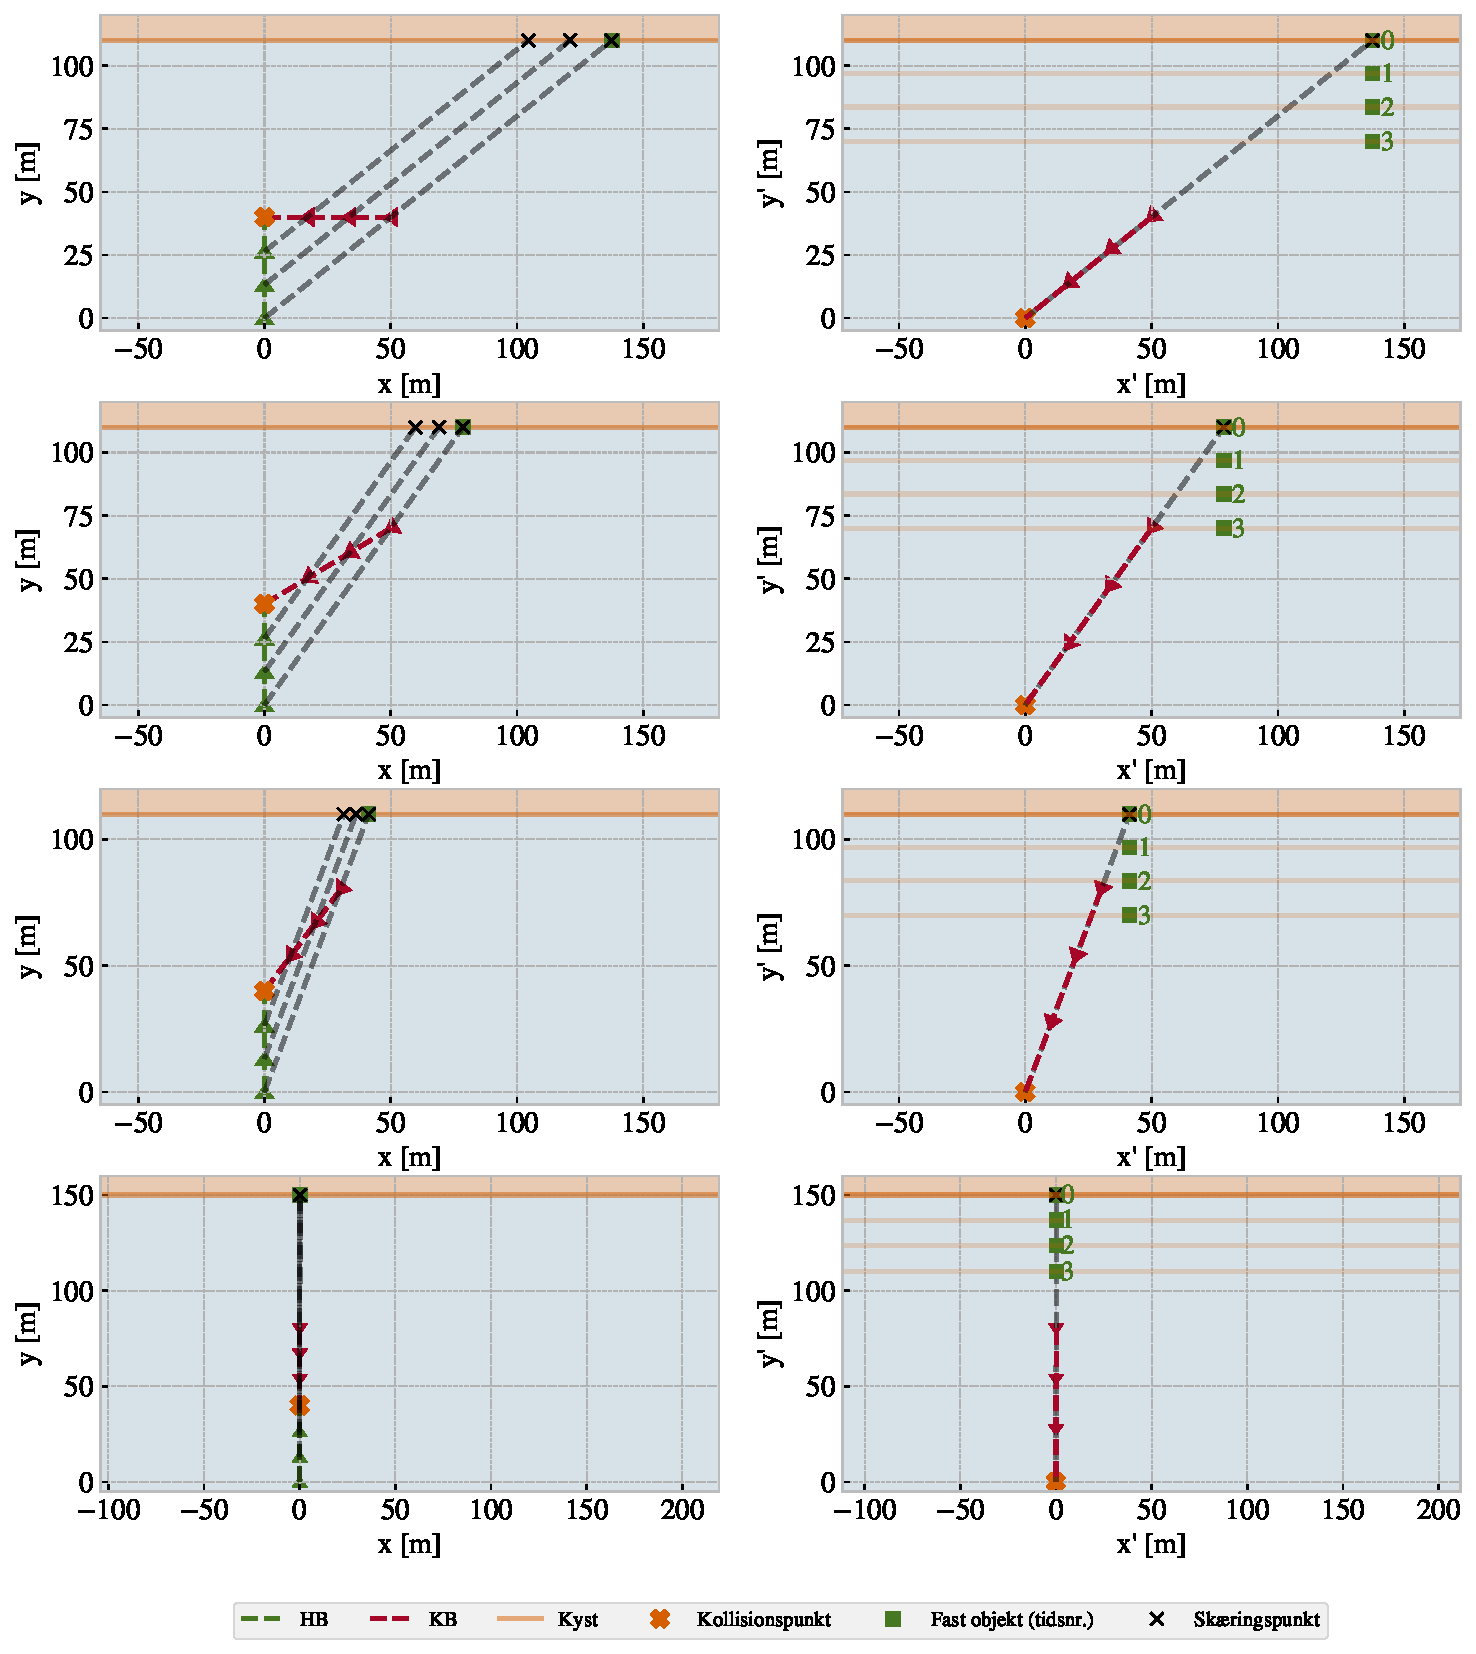
\includegraphics[width=\linewidth]{figures/subplot_C2.pdf}
  \caption[A table inside a caption]{
\begin{tabular}{|c|c|c|c|c|}
\hline
Figurrække & $HB_{start}$  & $KB_{start}$ & $HB_{slut}$ & $KB_{slut}$\\ \hline
1  & (0,0) & (50,40) & (0, 40) & (0, 40) \\ \hline
2  & (0,0) & (50,70) & (0, 40) & (0, 40) \\ \hline
3  & (0,0) & (30,80) & (0, 40) & (0, 40) \\ \hline
4  & (0,0) & (0.1,80) & (0, 40) & (0, 40) \\ \hline
\end{tabular}}
  \label{fig:subplot_C2}
\end{figure}


\clearpage
\subsection{Simmuleringer uden kollision}
\begin{figure}[H]
  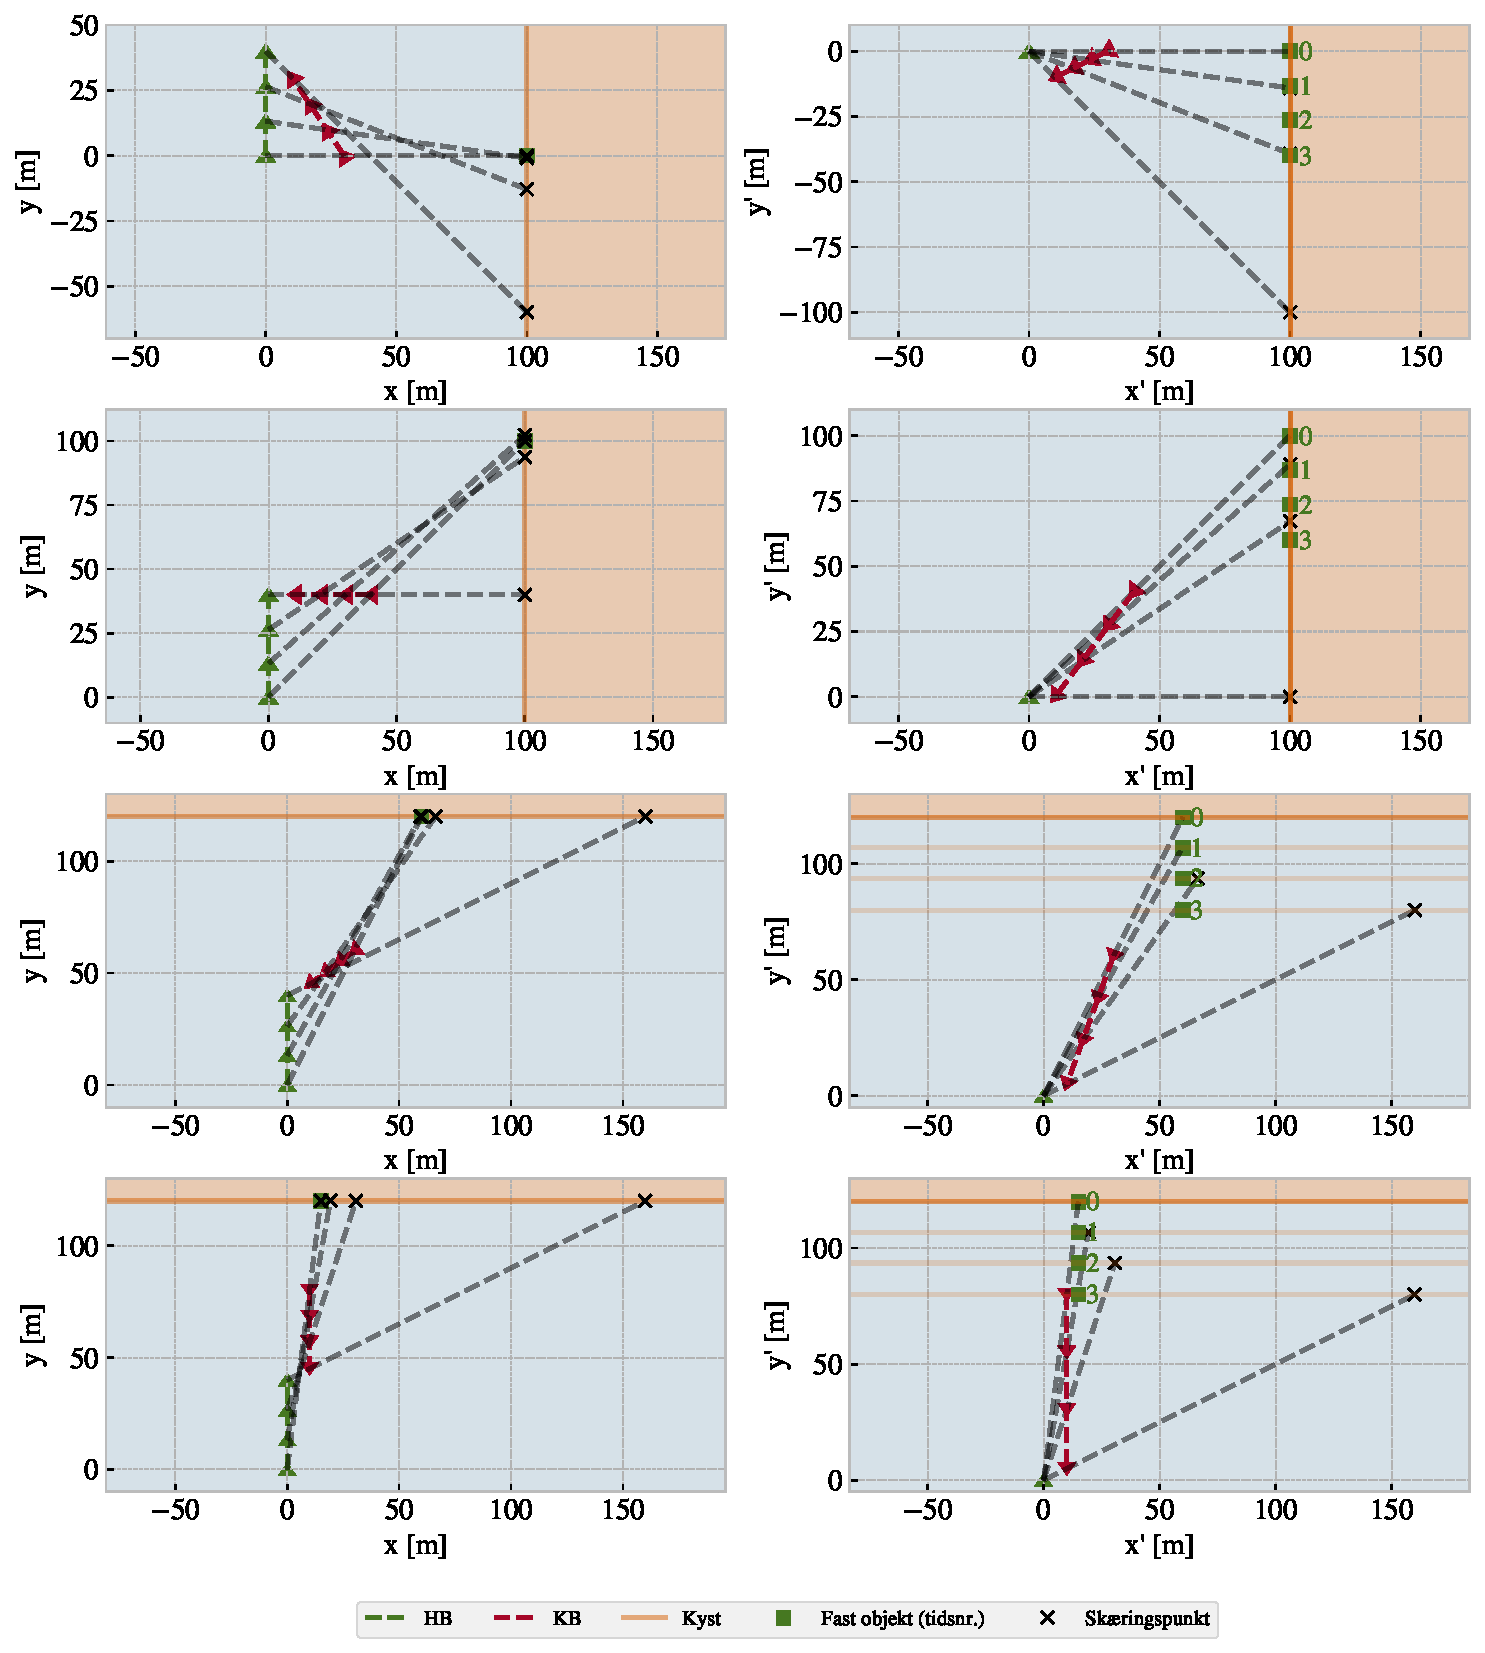
\includegraphics[width=\linewidth]{figures/subplot_NC1.pdf}
  \caption[A table inside a caption]{
\begin{tabular}{|c|c|c|c|c|}
\hline
Figurrække & $HB_{start}$  & $KB_{start}$ & $HB_{slut}$ & $KB_{slut}$\\ \hline
1  & (0,0) & (30,0) & (0, 40) & (10, 30) \\ \hline
2  & (0,0) & (40,40) & (0, 40) & (10, 40) \\ \hline
3  & (0,0) & (30,60) & (0, 40) & (10, 44) \\ \hline
4  & (0,0) & (10,80) & (0, 40) & (10, 44) \\ \hline
\end{tabular}}
  \label{fig:subplot_NC1}
\end{figure}








\end{document}
